\documentclass{article}
\usepackage{graphicx}

\title{Minesweeper is Hard}
\author{William Y. Feng}

\begin{document}

\maketitle
My friend keeps sending me half-finished minesweeper grids and challenging me to solve them:
\begin{center}
    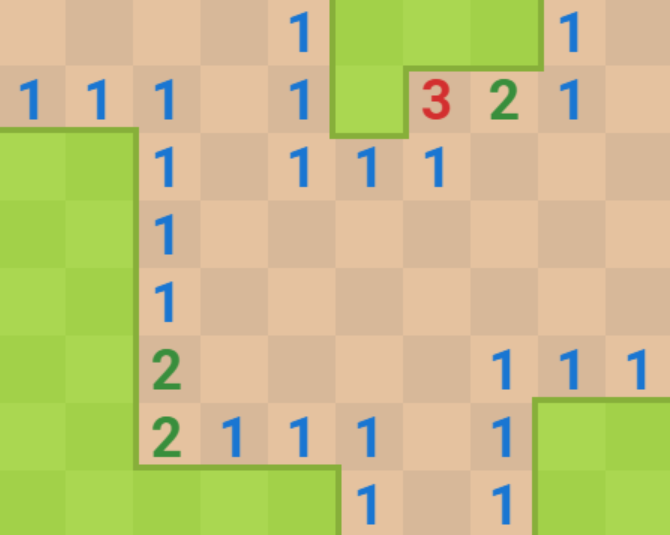
\includegraphics[width=2in]{images/Minesweeper_fig1.png}
    
    \small{A half-finished Minesweeper grid}
\end{center}

The thing is, my friend likes to mess with me sometimes, so I’m not convinced that it’s even possible to place mines on the grid in a way that’s consistent with the numbers. I want a fast way to check that any grid my friend sends me is solvable---specifically, I want a computer program that takes an $n \times n$ grid representing a partially-complete minesweeper grid as input and outputs whether there exists a configuration of mines consistent with the numbering. This problem is called MINESWEEPER. It’s important to note that the program doesn’t have to tell me what, if any, placement of mines makes the numbers consistent, simply a  “YES” or “NO.” (If my friend isn’t trolling me, then the task of finding a placement of mines can be left up to me.)

I also want the number of operations the program does to be bounded by some polynomial in $n$. This is a really loose bound, but it’s a nontrivial one---imagine a program that simply enumerates all possible ways to assign mines to the unrevealed squares and checks whether any assignment works. This could take up to the order of $2^{n^2} \cdot n^2$ operations, which is definitely not a polynomial in $n$. Such a program is said to run in polynomial time or to be a poly-time algorithm.

\subheader{CIRCUIT-SAT}

I might not have a program that can solve this problem in polynomial time, but I do have a magic box that takes in any arbitrary logic circuit as input and instantly determines whether there exists some combination of input bits that results in the output bit being 1. This problem is called circuit satisfiability, or CIRCUIT-SAT for short. For instance, if I put this circuit into the magic box:

\begin{center}
    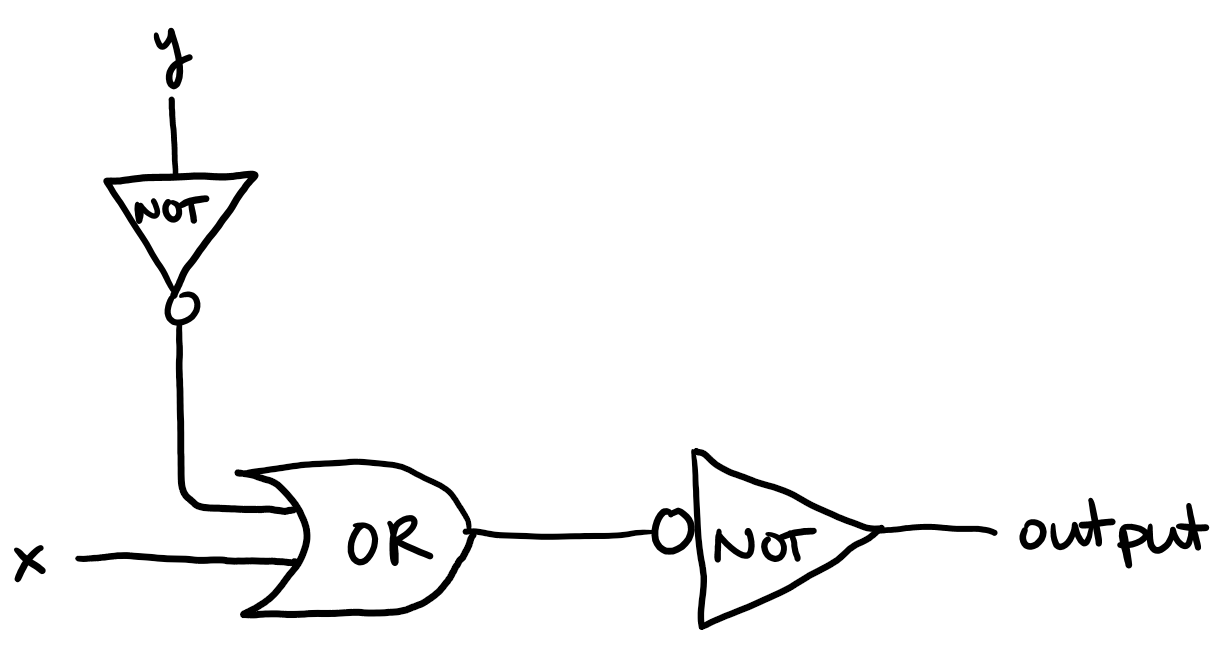
\includegraphics[width=2in]{images/Minesweeper_fig2.png}
    
    \small{Sample logic gate}
\end{center}

Then it will tell me, in a single operation, that the answer is YES. If we set $x=0$ and $y=1$, then the output will be 1 as well. The box won’t tell me what combinations of inputs will output a 1, it just tells me YES or NO. Using this magic box, I’m able to easily determine if one of my friend’s minesweeper grids is solvable. Here’s what my proposed program does:
\begin{enumerate}
\item Receives as input an $n \times n$ minesweeper grid
\item Write a sub-program in C where:
    \begin{enumerate}
    \item The input consists of proposed locations for mines in the grid
    \item The output is a binary representing whether the input is consistent with the grid
    \end{enumerate}
\item Compile this C code to a circuit using a C to HDL tool
\begin{enumerate}
    \item The compiled circuit takes in proposed locations for mines encoded in binary and outputs whether the input is consistent with the original grid
\end{enumerate}
\item Plug this circuit into my magic box and output its result
\end{enumerate}

You’ll have to trust me that the circuit resulting from step 3 has a polynomial number of gates in terms of $n$, but intuitively, since we’re only looping through every cell in the grid once and doing 8 checks per grid, the circuit should be relatively small.


\subheader{Going the other way}

To get revenge on my friend, I send them a large logic circuit with several inputs and one output, and challenge them to determine whether there exists some combination of input bits such that the output bit is a 1. Here’s the circuit I sent them:

Unlike me, they don’t have a magic box that can immediately tell them the answer. But, unlike me, they’re actually good at minesweeper and can instantly tell whether a partially-filled minesweeper grid has a solution just by looking at it. So here’s what they did:

\begin{center}
    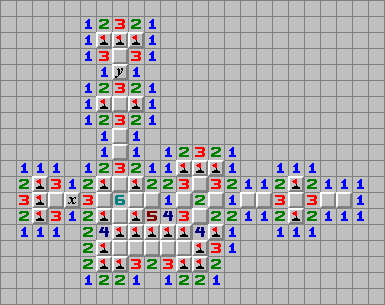
\includegraphics[width=2in]{images/Minesweeper_fig3.png}
    
    {\small When life gives you logic circuits, turn them into \href{http://www.formauri.es/personal/pgimeno/compurec/Minesweeper.php}{minesweeper grids}}
\end{center}

Dark grey cells are assumed to be 0, and flagged cells must logically have mines in them. The rightmost flag corresponds to the output wire, the square labeled $x$ on the left side of the grid corresponds to input wire $x$, and the square labeled $y$ near the top corresponds to input wire $y$. Reasoning out the grid, we can determine that the output square has a mine if and only if the logical statement “not ($x$ or not $y$)” is true, which corresponds exactly with the logical circuit I gave my friend.

In fact, my friend is able to convert any logic circuit into a minesweeper grid using some simple “widgets” representing wires and all the different kinds of gates. Furthermore, it only requires a grid size that’s polynomial in the number of gates in the circuit. This, together with their superhuman minesweeper-solving skills, allows them to solve any logic circuit I present to them in polynomial time.


\subheader{Closing remarks}

This was a brief introduction to complexity theory, and in this article we showed (non-rigorously) that the two problems MINESWEEPER and CIRCUIT-SAT (short for circuit satisfiability) can be used to solve one another. There are a lot of unsolved problems in this field, such as the famous P=NP conjecture, and if this article was interesting, I recommend looking into it further with the resources.
}
\end{document}